\chapter{相关技术介绍及研究动机}
\section{分布式并行图处理框架}
由于MapReduce编程范式存在着进行多轮迭代图计算时带来中间结果存储开销,实现图算法需要额外转换等问题,
人们在并行分布式处理大规模图数据过程中广泛使用BSP(Bulk Synchronous Parallel)模型\cite{bsp@1990}。
BSP模型是图灵奖得主Valiant于1990年提出来的一种基于消息通信的并行计算模型,
其核心思想是将一个巨大的计算任务分解为一系列的迭代运算,因此尤其适合做数据的迭代计算。
如图\ref{fig:bsp}所示,一个BSP作业由若干个顺序执行的超步(super step)组成:$S_1,S_2,\cdots,S_n$,对应于$n$次迭代处理。
并行任务按照超步组织,在超步$S_i$内,各任务异步接受来自$S_{i-1}$的消息,执行本地计算并发送消息给下一个超步$S_{i+1}$。
在超步之间,通过显式地同步控制,确保所有任务均已完成超步$S_i$的工作,这种同步方式可避免死锁和数据竞争问题。
BSP模型避免了MapReduce模型在多次迭代时的数据反复迁移和作业连续调度,其特有的超步和全局同步机制使得迭代处理的控制更加灵活。

\begin{figure}[!htbp]
  \centering
  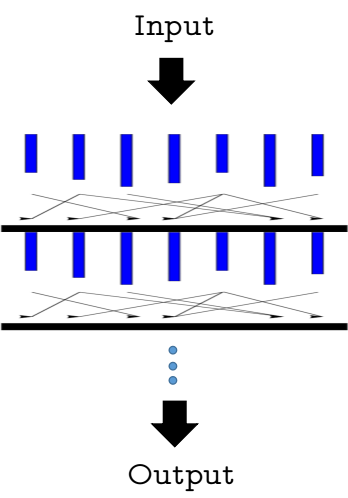
\includegraphics[width=0.40\textwidth]{bsp}
  \bicaption{BSP模型}{bsp model}
  \label{fig:bsp}
\end{figure}

受BSP计算模型的启发,Google在2010年首次提出了以顶点为中心的分布式图计算框架Pregel\cite{Malewicz@SIGMOD10}。
自Pregel之后,围绕着Pregel存在的局限性,以及新的问题和需求,人们又开发出了一系列新的用于处理大规模图数据的分布式并行计算框架。
这些框架在以下四个主题方面上存在着不同。

\subsection{任务调度机制}
任务调度是分布式图处理系统必须解决的问题。根据迭代计算过程中每个超步之间是否有明确界限,或者说不同超步之间是否交错运行,
可以将分布式图计算框架所采用的调度模式分为3种:\textit{同步调度模式,异步调度模式,混合调度模式}。

在同步调度模式中,两个相邻迭代之间存在同步控制机制,需要在当前迭代结束后才能进入下次迭代。
在这种模式下,执行运算的图节点所能看到的数据是上次迭代所有节点执行更新后的结果数据。
同步调度模式控制机制简单,便于用户理解且具有较强的表达力。
在采用同步调度模式的系统上运行图算法,运行过程及结果是确定的,这有助于同步程序的设计、调试和部署。    
虽然同步调度模式在简单易用和扩展性方面表现良好,但也存在多方面的不足:
(1) 计算节点之间的同步会产生额外的开销。
(2) 由于计算节点处理能力不同或者图数据划分不均匀,会导致在处理同一迭代时不同计算节点执行运算的时
间差异很大,因同步的存在使得处理最慢的节点成为该次迭代的瓶颈,从而产生木桶效应。
(3) 在同步模式下,两次迭代之间,消息的传播只能发生在直接邻居节点,这种低效的传播方式使得同步算法在某些应用下不能够有效收敛。
为解决同步模式中的这些问题,科研工作者提出了异步调度模式和混合调度模式。

在异步调度模式中,两次迭代之间没有明确的界限,活跃图节点只要接收到其需要的消息,
不需要等待其他所有图节点就可以动态地接受调度器的调度执行,并向其他图节点广播计算结果。
在异步调度模式中,因为摒弃了同步路障阶段,所以能够有效减少同步模式中木桶效应的影响。
尽管异步调度模式可以提高某些算法的性能,但是该模式仍然存在多方面的不足之处。
(1) 异步调度模式的分布式图处理系统设计相较于同步系统来说更加复杂,系统除了要设计正确高效的调度器之外,
还要解决异步计算过程中对数据的读写访问冲突等问题。
(2) 异步调度的计算过程和结果具有不确定性。
(3) 相较于 Pregel 等同步系统来说,异步调度的编程难度有所增加,并且程序的异步执行对算法的调试也提出了更高的要求。

在深入分析同步和异步调度模式系统的优缺点后,许多学者提出了混合调度模式的调度机制,PowerSwitch\cite{Xie@PPoPP15}是这方面比较有代表性的系统。
在不同调度模式下,图算法的执行算效率受到图应用算法、图划分方式、迭代执行进度、输入图的特性以及集群状态等多方面的影响。
因此,PowerSwitch 通过一组启发式的算法建立代价收益模型来动态预测同步模型和异步模型两种调度方式的性能,并实现在计算过程中对两种模型的自由切换。
实验结果表明,PowerSwitch 可以准确预测两种模型的性能,并且快速地完成调度模式切换,相比于使用单一的调度模式,
在其上执行的大量图算法,如 PageRank、单源节点最短路径等,都在执行效率上得到不同程度的提高。

\subsection{通信机制}

目前,常见分布式图处理系统所采用的通信方式主要可以分为两类:\textit{基于共享内存的方式和基于消息传递的方式}。
        
在基于共享内存进行通信的分布式图处理系统中,每个图节点的数据以共享变量的方式存储在计算节点上,
当某活跃图节点在计算过程中需要其他节点数据时,可以直接按照相应的内存地址进行读取。
在分布式环境中,因每个计算节点都有自己独立的内存地址且需要保持数据的一致性,
所以使得共享内存的通信方式实现起来变得较为困难。
为有效地管理集群中各个计算节点的内存地址,微软推出的分布式图计算框架 Trinity\cite{Shao@SIGMOD13}设计了一套有效的集群内存管理方案。
该方案将集群内每个计算节点的内存组织成一个巨大的虚拟内存空间,并按照一定模式给予每个存储单元一个 64 位的存储空间地址,
存储在集群内的任意图节点都可以使用该存储空间地址访问虚拟内存空间中的任意单元,从而使得集群共享内存通信在形式上与单机环境类似。

在基于消息传递的方式当中,图节点之间的信息交互通过利用网络通信平台在节点之间发送消息来实现,消息中包含要传送的数据和目标顶点 ID。
在这种方式中,图节点在计算过程中会根据运算逻辑产生相应的消息并发送到目的节点。
如果目的节点和源节点位于同一台机器上,则直接将该消息放到相应图节点的消息队列中;
否则,将该消息放置到消息发送缓冲池中等待发送。
在消息的发送过程中,系统会使用批量发送的方式来优化网络通信。

鉴于在分布式图处理系统中,通信代价严重影响整个系统的性能,对通信方式进行优化以减少消息的时空和网络开销显得格外重要。
在过去的研究中,主要出现了两种优化方式:
第 1 种是通过合理的图分割技术降低图分区之间的连通性,减少跨机器的通信请求,
虽然该方式不能够减少消息的存储空间,但可以从根本上减少跨机器的消息数量。
第 2 种是通过 Combine、Receiver-side scatter 等技术减少消息数量,降低网络开销。
Combine 机制会将发送到相同目的顶点的消息合并成一条,在降低网络开销的同时减少消息的存储开销。
Receiver-side scatter 技术是对发往同一目的机器不同目的节点的消息进行合并处理。

在系统进行消息传递通信的过程中,根据信息的流向,又可以把分布式图处理系统的工作模式划分为\textit{push模式,pull模式}两种类型。

在 Push 模式中,信息由当前活动图节点流向邻居节点,即,当前活动图节点完成计算并产生相应的数据信息后,数据信息按照出边传输到相应邻居顶点。
在内存资源充足的条件下,该工作模式允许各个计算节点高效并发地对图节点进行处理,
但是该模式需要消息产生后立刻发送到目的节点,并要目的节点对消息进行存储,增加了系统对内存的需求。

在 Pull 模式中,信息由邻居节点流向当前活动图节点,即,当前活动图节点在计算过程中需要数据信息时会按照入边向其邻居节点请求数据。
在 pull 模式下,因为图节点请求到数据后会立刻参与计算并释放对应的消息,所以可以避免存储大量的消息,减少系统对内存的需求。
然而在消息传递方式下使用 Pull 模式时,增加了额外的通信请求开销。

Push 和 Pull两种模式各有利弊,分别适合不同的场景,显然, 将两种模式有机地结合起来才是最优选择。
单机图计算系统Ligra\cite{Shun@PPoPP13}采用了这种混合策略, 根据需要参与计算的边数自适应地在两种模式间切换。
Gemini\cite{Zhu@OSDI16} 则将这种双模式计算引擎从单机的共享内存扩展到了分布式环境中,
并且进一步将两种模式下的计算过程都细分成发送端和接收端两个部分,从而将分布式系统的通信从计算中剥离出来。

\subsection{图划分}

图数据划分是进行分布式图处理的基础,划分结果的好坏严重影响着分布式图处理系统的性能。
一个有效的图划分策略能够在使整个系统达到负载均衡的同时,尽可能地减少网络开销。
在图划分过程中应遵循两个重要的原则:首先是降低划分后子图之间的连通性,以降低网络开销;
其次是保证子图大小均匀,以实现系统的负载均衡。
图计算框架中的图划分技术可以从\textit{图划分方式和图划分策略}两个方面进行论述。

分布式图处理系统在对图数据进行划分时,主要采用了两种划分方式:
边切分方式(vertex-cut)\cite{Gonzalez@OSDI12}和点切分方式(edge-cut) \cite{Malewicz@SIGMOD10}。
边切分指在图的划分中对其边进行切分,图数据被划分后,图中每一个节点出现且仅出现在一个子图中,
被切断边的两个顶点将出现在两个不同的子图中。
点切分是对图的节点进行切分。图数据被切分后,图中的每一条边出现且仅出现在一个子图中,邻居多的点将会出现在多个子图中。

在图划分策略方面,分布式图处理系统主要有3种:\textit{离线划分策略、流式划分策略以及动态重划分策略}。
离线划分策略是使用离线图划分算法,在图数据被分布式图处理系统加载前将其划分为若干子图。
流式划分策略是在数据加载过程中对图数据边加载边划分,其假定数据以节点流或者边流的方式到达,
在划分过程中,按照已到达数据的分布信息,通过一组启发式的规则来决定当前到达数据的划分位置。
在分布式图处理系统的运行过程中,造成负载不均的因素有很多,括初始图数据划分不均、集群环境的改变、活跃节点数目的变化等。
为此,许多系统都设计了相应的动态重划分策略来保证负载均衡。

\subsection{计算粒度与顶点计算模型}

当前,图计算系统在对图数据进行遍历计算的过程中主要使用了3种不同的计算粒度:\textit{以顶点为计算粒度,以子图为计算粒度和以路径为计算粒度}。
    
以顶点为计算粒度的分布式图处理系统其迭代处理过程通过对图节点的遍历完成,这种模式逻辑简单且具有良好的算法表达能力,
因此这种模式被绝大多数框架如GraphLab\cite{Low@12}、GraphX\cite{Gonzalez@OSDI14}、Giraph\cite{Avery@HS11}等采用。
不过该模式牺牲了图节点访问同一分区其他节点信息的灵活性,因此存着着收敛速度过慢,网络通信量大等缺点。

针对以顶点为计算粒度模式的缺点,人们又提出了大量以子图为计算粒度的分布式图处理系统,如GraphHP,GoFFis等。
这种模式先对子图的边界点进行处理,然后接着处理子图内部的节点,不过这种模式表达能力较弱,因此不能够取代以顶点为粒度的模式。

以路径为计算粒度的模式主要在单机集中式图处理系统中使用,这种模式将边数据和点数据进行分区,
对边采用顺序访问的方式进行遍历计算,减少了对边数据的随机访问,进而降低了磁盘访问开销。
目前为止,在分布式环境下以路径为计算粒度的模式还缺少有效实践,不过这种模式可以为分布式图计算框架中的某些优化提供借鉴意义。

绝大多数分布式图处理系统以顶点为计算粒度,用户需要以图中的节点为粒度定义运算函数。
在实现运算函数的时候,人们采用的是"Think Like A Vertex"\cite{TLV}这种编程思想。
% 这个运算函数的功能包括消息的收发、节点值的更新以及顶点状态
% 的改变等。然后,系统按照该运算函数对图中的每一个顶点进行同步或者异步的更新运算。      
这种编程思想以顶点为中心,从顶点的角度出发去描述图计算过程中每个顶点的行为。
在编程框架的迭代过程中,图中所有顶点不断地执行用户定义的顶点程序(vertex program),每个顶点只能从邻居顶点发送或接收消息,
当顶点收到消息后就处于激活状态,图计算的过程就是维护和更新每个顶点的状态的过程,当所有顶点都已经处于非激活状态,系统结束计算过程。
在具体实现过程中,\textit{计算框架可以把顶点程序分解为一个,两个或三个执行阶段}。

单执行阶段的顶点程序可以用一个计算函数来表示,这个计算函数遵循这样的执行流程:访问邻居数据和消息,计算新的顶点状态值,分发状态变化值。
Pregel是采用了这种顶点程序抽象的一个典型代表。
两阶段的顶点程序常被分解为 Scatter-Gather 两个函数,并被称之为 Scatter-Gather 模型,
其中scatter阶段用于把顶点值分发给顶点,gather阶段用于收集输入然后用于执行顶点更新,
GraphChi\cite{GraphChi}使用Scatter-Gather作为标准的编程模型。
此外GRE\cite{GRE}编程框架也提出了一种在消息传递中使用的两阶段编程模型,Scatter-Combine,这种方法在活跃消息中既传递数据也传递操作。

PowerGraph\cite{Gonzalez@OSDI12}提出了一种三阶段执行过程的顶点程序,Gather-Apply-Scatter(GAS)。
Gather阶段对所有输入顶点或边上的消息进行求和,这个结果在Apply阶段用于更新顶点的状态,Scatter阶段把更新的消息传播出去。
PowerGraph是由共享内存架构的GraphLab\cite{Low@12}发展而来的,它既支持基于BSP实现的同步引擎,也支持采用灵活调度策略的异步引擎。
PowerGraph通过GAS的顶点编程模型配合vertex-cut的图划分方法,提高了图并行处理的粒度,较好地解决了图的幂律分布带来的计算不平衡问题。
在PowerGraph的vertex-cut划分方法中,图按边划分,每条边被唯一地分配到某个机器上去,顶点则在机器之间存在副本。
迭代过程中,每个顶点的副本能够互相独立的执行本地的gather阶段,然后各个副本把执行结果发送到指定好的master顶点上,
master顶点使用这个结果来执行完Apply阶段后把结果再发送给各个副本,然后各个副本又可以独立地执行本地的scatter阶段。


\begin{figure}[!htbp]
\centering
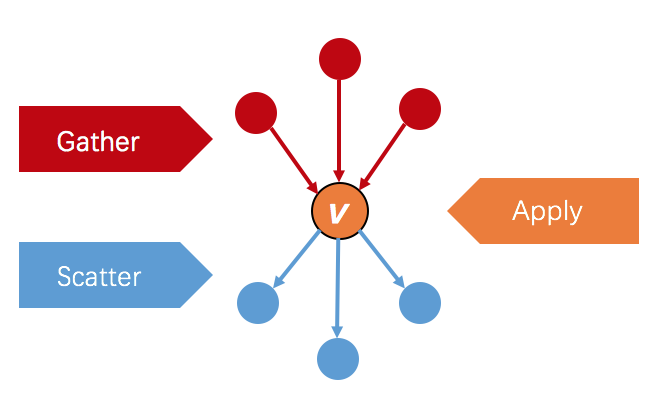
\includegraphics[width=0.40\textwidth]{gas_user}
\bicaption{用户视图下的GAS模型}{GAS Model in User View}
\end{figure}

在GAS的编程模型中,副本点的存在使得分布式图计算系统能够在多台机器上并行地处理顶点的计算以及在本地访问远程的邻居顶点,
但是副本点也带来了数据一致性和副本点之间的消息传递问题,这些问题会在迭代计算过程中带来频繁的全局同步和通信开销,
LazyGraph\cite{Wang@PPoPP18}提出了一种 延迟数据一致性(lazy data cohereence) 的方法,将一个顶点的不同副本当作是独立的顶点,
它们可以维护和更新自己的数据,各自独立地进行本地计算,系统会选择合适的时间节点在副本点之间进行全局消息交换然后通过计算来使得它们达到数据一致性,
这种方法消除了顶点计算过程中副本点之间的数据一致性和消息传递开销,减少了副本点之间消息交换的次数,极大地减少了系统中全局同步的次数和网络通信量。
副本点之间进行全局消息交换的时间节点直接影响着系统的性能,LazyGraph使用机器学习模型训练出的参数选择具体的时间节点。

% 自Pregel之后,研究者们使用各种优化手段提出了众多的分布式图计算框架。
% 这些框架大多数都对同一个顶点的不同副本点采取 eager datacoherency 的方式,因此带来频繁的全局同步和通信。 
% LazyGraph 采用 lazy data coherency 的方法来解决这个问题。
% Hieroglyph\cite{ju2017hieroglyph}也同样使得同一顶点的不同的副本点可以独立本地更新自己的数据。
% 但是,Hieroglyph关注于将计算从通信中解耦出来,以获得充足的本地计算,并且需要用户定义模块来解决数据一致性的问题。
% 而 LazyGraph 则关注于延迟副本点间的数据一致性,并同时减少全局同步次数和网络通信,并且在编程框架内部自动地维护副本点之间的数据一致性。
% 因此现有的研究不能直接用于处理我们提出的延迟数据一致性方法中遗留的几个问题。

\section{基于延迟数据一致性方法的 LazyGraph 图计算系统}
\subsection{顶点副本的延迟数据一致性方法}
% 延迟数据一致方法是什么

% 副本点
副本点在分布式并行图计算框架中发挥了巨大作用。
一方面它可以使得集群的多台机器对一个顶点进行并行处理,提高了计算效率。
另一方面,副本点使得顶点能够在通过本地内存直接访问那些被划分在远程机器的顶点,减少了通信开销。
图\ref{fig:graph_cut}给出了一个图在三台机器上分别进行点划分和边划分的结果。
可以看到无论哪种方式,图中的顶点都会产生副本点。
以边划分为例,图\ref{fig:edge_cut}中C顶点在2号机器上有一个副本,
这使得系统可以对C顶点的两条边C-B和C-D进行并行处理。
此外,由于C顶点在2号机器上的副本点的存在,2号机器上的B顶点在访问它的邻居C顶点时可以从本机内存中直接访问,
而不必通过网络请求从3号机器上访问。



\begin{figure}[!htbp]
  \centering
  \begin{subfigure}[b]{0.35\textwidth}
    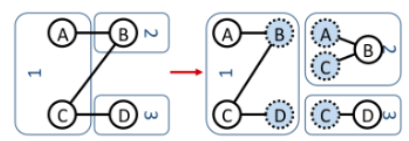
\includegraphics[width=\textwidth]{vertex_cut}
    \caption{}
    \label{fig:vertex_cut}
  \end{subfigure}%
  ~% add desired spacing
  \begin{subfigure}[b]{0.35\textwidth}
    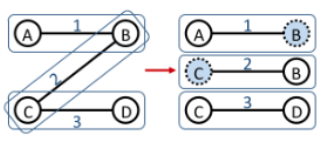
\includegraphics[width=\textwidth]{edge_cut}
    \caption{}
    \label{fig:edge_cut}
  \end{subfigure}
\bicaption{点划分和边划分}{vertex-cut and edge-cut}
\label{fig:graph_cut}
\end{figure}

% eager data coherence 及其 冗余

副本点在带来巨大好处的同时也引入了数据一致性的问题。
对于一个顶点在集群中同时分布存在的多个副本,之前的多数分布式图计算编程框架都采用 eager data coherency 的方式来维护
这些副本之间的数据一致性。
这种方式要求对顶点的任何修改都要在下一次新的修改之前同步到其他所有副本上。
图\ref{fig:pg-eager}表示了典型的图计算框架PowerGraph是如何实现 eager data coherency 的。
在PowerGraph的实现方式中,顶点的多个副本中某一个被标记为 master 点。对顶点的修改只在 master 点上进行,
修改之后把master 点的最新状态通过网络同步拷贝到其他副本点上。

\begin{figure}[!htbp]
  \centering
  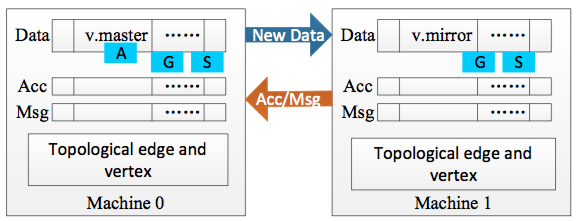
\includegraphics[width=0.40\textwidth]{pg-eager}
  \bicaption{PowerGraph 的 eager data coherency 实现}{Eager Data Coherency in PowerGraph}
  \label{fig:pg-eager}
\end{figure}

Eager data coherency 方式虽然最大程度的维护了顶点上数据的原子性,但是却带来了大量的冗余。
由于副本点上的数据必须从 master 上拷贝而来,因此在 master 上的数据进行修改时副本点上无法进行计算,
这带来了冗余的等待。
同时,由于master点上的数据必须通过网络同步拷贝给其他机器上的副本点,系统中因此引入了大量频繁的全局同步和通信。

% lazy data coherence 的方法
针对 eager data coherency 存在的问题,我们另外提出了一种称之为 LazyAsync 的迟数据一致性方法。
这种方法在保留副本点带来的好处的同时避免了 eager data coherency 方法存在的各种冗余问题。
在 LazyAsync 方法中,每个副本点都被当作一个独立的顶点,并且各自可以拥有自己的本地数据。
顶点在不同机器上的副本点分别维护着自己不同的本地视图,并且基于公式
$x_{i}^{t+1}=x_{i}^{t}+_{o p} \oplus_{j \rightarrow i \in E} \Delta_{j}^{t}$
进行迭代更新。
虽然不同的副本点它们收到的消息的次序不一致,但是只要有相同的初值和消息和,它们最终能够得到一致的值。

LazyGraph 将副本点 $v_1,v_2,\cdots,v_k$ 的计算过程分为本地计算和数据一 致性两个阶段。
其仅仅在数据一致性点的时候将各自的本地消息和其它副本 点的远程消息进行合并,再通过计算得到数据一致性。
因此,LasyAsync 的模式使得副本点在相邻两个数据一致性点之间维护各自不同的本地视图,
并在 数据一致性点的时候得到一致的全局视图。


LazyAsync 保留了现存分布式图计算编程框架的编程接口,同样使用GAS模式,
但是,需要用户将原来点程序改为 pull-style 模式并支持 deltaMsg 消息传递。
和现存的分布式图计算编程框架一样,在有向图$G = \{V, E\}$上用户定义一个点程序 P,然后图中所有顶点$v \in V$并行地在多台机器上进行计算。
顶点之间的通信直接通过给对方发送消息来完成。一个顶点可以接受其它点发送过来的消息,然后修改自己的数据,再发送消息给其它顶点。
而图中的边用来传输数据。


当然,LazyAsync 也有和现存的分布式图计算编程框架存在区别。
LazyAsync 要求顶点的迭代计算是可以用公式 $x_i^{t+1} = x_i^t +_{op} \oplus_{j \rightarrow i \in E} \Delta_j^t$ 来表示,
其中,$i$为顶点的 id 号,$t$为迭代计数器,$+_{op}$和$\oplus$表示运算符,$\Delta_j^t$表示顶点$j$在第t次迭代的消息变化值(deltaMsg)。
此外,$\oplus$是由用户定义的消息累加的运算符,LazyAsync 要求它必须是可交换且可累加的。
在 Gather 阶段,顶点$i$收到邻居点发送给它的消息$\Delta_j^t$,然后用$\oplus$操作进行累加求和,得到累加和 accum。
然后在 Apply 阶段,中心点用自己的数据和刚刚求得的累加和 accum 进行迭代更新$x_i^{t+1} = x_i^t +_{op} accum$。
最后,在 Scatter 阶段,点$i$的变化值$\Delta_i^{t+1}$又通过边发送给其它相邻的顶点。


虽然在用户的视图下,其定义的点程序$P$定义在图$G = \{V, E\}$中的顶点上,
但是在分布式的编程框架中,$P$ 是运行在每台机器上被划分后的子图上的。
在图的加载到分布式环境的过程中,LazyAsync 使用点划分的形式将顶点划分开,若干的顶点产生副本点并横跨在多台机器上。
运行时系统能将用户定义的点程序 P 转变为更低层次的图操作,再使用 LazyAsync 来并行异步地执行顶点的计算。

在以下的内容中,我们将介绍如何用 Lazy Data Coherency 去并行异步地进行顶点的计算。
LazyAsync 重新定义了在运行时系统中,副本点$v_0, v_1, ..., v_k$如何进行计算,并得到顶点的值。
如图\ref{fig:lazy_data_coherency}所示,
LazyAsync 将在分布式环境下副本点$v_0, v_1, ..., v_k$的计算分为本地计算(local computation statges)和数据一致性阶段(data coherency stages)。
在本地计算阶段中,同一个顶点的副本点维护着各自不同的本地视图,然后用在同一台机器上从本地的邻居顶点收到的本地消息更新自己的数据。
顶点的新的本地视图对于本地的邻居顶点而言是立即可见的,而不用等待数据一致性点。
在本地计算的同时,所有的副本点都会累加从本地邻居点发送过来的变化信息。
而在数据一致性阶段,每个副本点都会把自己的消息变化的累加和通过网络发送给远程的其它副本点,并接收其它副本点发送过来的消息累加和。
之后,所有接收到消息的副本点都在自己原本的本地视图和其它副本点发送过来的消息和执行 Apply 操作,最终达到一致的全局视图。
\begin{figure}[!htbp]
\centering
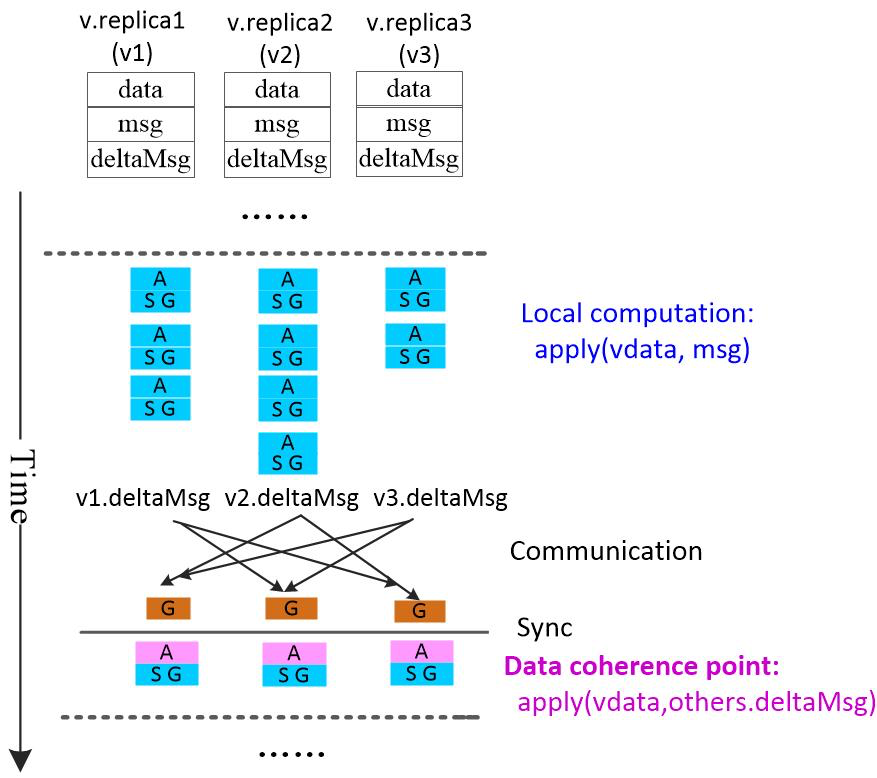
\includegraphics[height=12cm]{lazy_data_coherency.png}
\bicaption{点$v$的延迟数据一致性过程}{Lazy Data Coherency for replicas of v}
\label{fig:lazy_data_coherency}
\end{figure}

\subsection{延迟数据一致性方法的开启策略}
% 现有的开启策略,及不足之处

数据一致性节点的选择,也就是 延迟数据一致性方法的开启策略, 是 LazyAsync 的重要组成部分。
% 延迟数据一致性方法要解决的一个重要问题就是它的开启策略。
在把迭代公式修改为差值累加的形式之后, LazyAsync 方法正是通过延迟数据一致性的方法来减少冗余的通信和同步。
而延迟数据一致性方法的开启策略要解决的就是系统何时进行延迟数据一致以及延迟数据一致持续多久的问题。
这个策略既不是越早越好,也不是越晚越好,过早开启或者过完开启都有可能得不到相对最优的性能提升。


在之前的工作中,我们采用了一个input-behavior-interval决策树模型来作为延迟数据一致性方法的开启策略。
如图\ref{fig:dtree}所示,这个决策树模型采用两个特征作为判断条件:

\begin{enumerate}
  \item 输入图的本地性(locality)。我们使用边和顶点的比例 $\frac{E}{V}$ 和复制因子 $\lambda$ 来表示图的输入图本地性。
  其中,复制因子 $\lambda$ 定义为整个图中所有顶点的平均副本点数,也就是总的副本点数于总的顶点数的比值。
  \item 图算法的运行时特征。大多数图算法都是迭代式地进行计算,不断的更新顶点的数据直至达到某个特定的收敛条件。
  在每一轮的迭代中,顶点的活跃点数\verb|vcnt| 是不断变化的。
  我们使用活跃顶点数的变化趋势来描述算法的特征。
  具体的,用如下公式进行计算:
  \begin{equation}
  \label{equ:chap04:trend}
  trend = \frac{vcnt^{t-1}-vcnt^t}{vcnt^{t-1}}
  \end{equation}
  我们在数据一致性阶段计算每一轮迭代时的活跃顶点数 \verb|vcnt|,如果 \verb|vcnt| 是负值,那么算法处于一个上升阶段,否则,则处于下降阶段。
\end{enumerate}

\begin{figure}[!htbp]
\centering
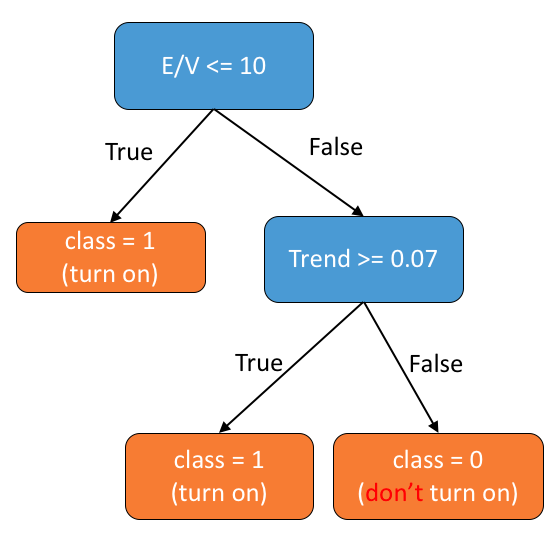
\includegraphics[width=0.40\textwidth]{decision_tree}
\bicaption{决策树模型}{Dceieson Tree Model}
\label{fig:dtree}
\end{figure}


input-behavior-interval 决策树模型是一个离线调优模型。
它的基本思路是先通过手动调优找到各种情况组合下的相对最优的延迟数据一致性的开启节点。
然后对这个过程中产生的大量数据集进行训练拟合。
最后把拟合得到的决策树模型反代入到系统实现中作为一个在线的判断策略。


input-behavior-interval 决策树模型并不能真正有效地解决 LazyAsync 的开启策略问题。
一方面在 input-behavior-interval 决策树模型的训练过程中需要手动选择各种特征点组合进行试错。
另一方为了得到训练数量数据,也需要事先在大量的算法和输入图组合上进行繁琐的手动调优。
最重要的是基于机器学习方法得到的优化方法存着固有的过拟合或泛化能力不足的问题。
实际的计算过程中如果遇到训练集和验证集中没有遇到过的例子,决策树模型指导下的LazyAsync可能无法得到相对最优的性能提升。
图\label{fig:dtfail}就给出了这样一个例子。

\begin{figure}[!htbp]
\centering
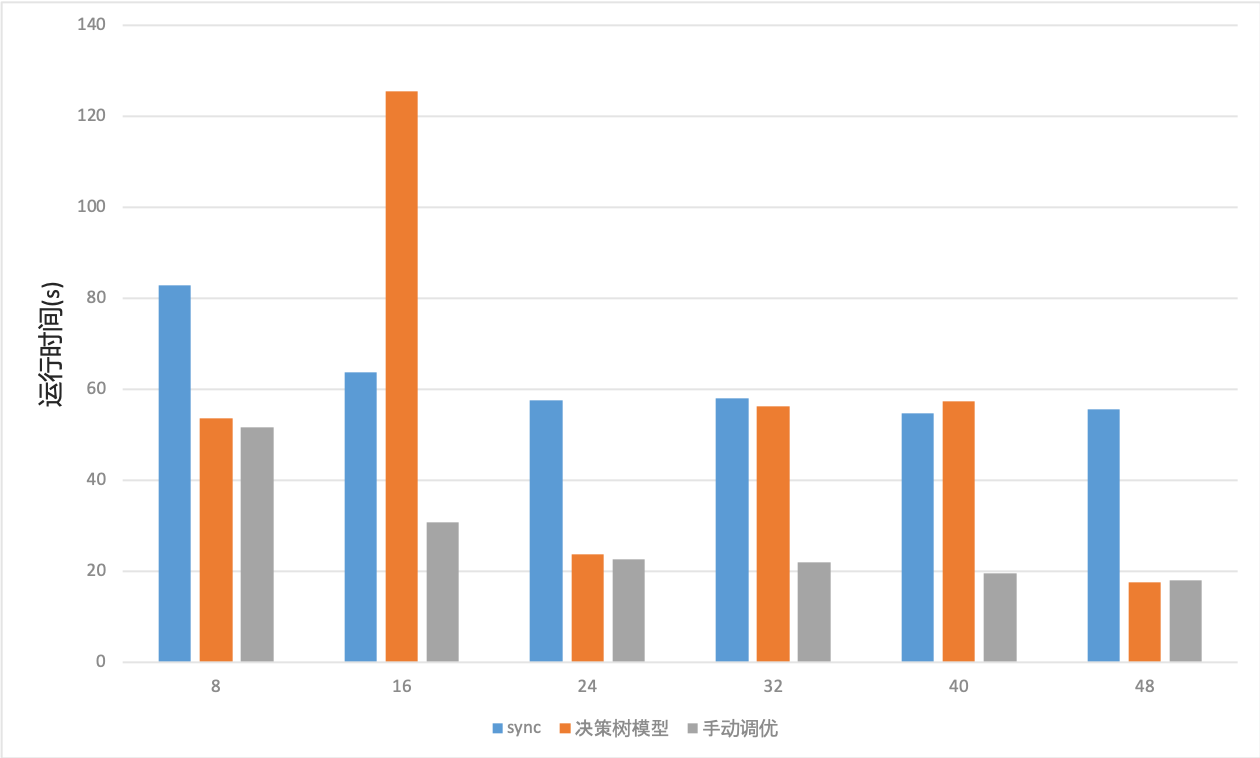
\includegraphics[width=0.40\textwidth]{dtreefail}
\bicaption{决策树失灵的情况}{Failure of decision tree}
\label{fig:dtfail}
\end{figure}

延迟数据一致性方法对副本上的数据进行延迟一致,
已经被证明为是一种行之有效的提升图计算执行效率的方法。
但是关于这种方法如何得到相对最优的性能提升这一问题还有待研究。
我们之前的工作中采用决策树的方法来解决 LazyAsync 的优化问题,
但是决策树模型一方面自身的训练需要一个繁琐的手动调优过程,另一方面也存在着失灵的情况,
因此并不能真正有效的解决这一问题。


自 Pregel 之后,研究者们使用各种优化手段提出了众多的分布式图计算框架。
这些框架大多数都对同一个顶点的不同副本点采取 eager datacoherency 的方式。
在相关工作中,Hieroglyph\cite{ju2017hieroglyph}也同样使得同一顶点的不同的副本点可以独立本地更新自己的数据。
但是,Hieroglyph 关注于将计算从通信中解耦出来, 以获得充足的本地计算,并且需要用户定义模块来解决数据一致性的问题。
而 LazyGraph 则关注于延迟副本点间的数据一致性, 并同时减少全局同步 次数和网络通信,并且在编程框架内部自动地维护副本点之间的数据一致性。 
因此现有的研究不能直接用于处理我们提出的延迟数据一致性方法中遗留的优化问题。


本课题通过进一步的实验,提出了一种基于解的局部性的自适应优化方法有效地解决了 LazyAsync 方法的优化问题。
本课题先是通过实验和理论分析,解释了LazyAsync 方法在不同的开启策略下得到不同程度的性能提升的现象。
并从有效计算的角度出发,论证了 LazyAsync 在避免了 eager data coherency 的冗余通信和同步的同时,
自身却有可能带来一定程度的冗余计算,因而无法得到相对最优的性能提升。

通过分析全局解和局部解的关系,我们进一步发现了图计算过程中解的局部性规律。
解的局部性规律可以用于指导延迟数据一致性方法减少冗余计算。
基于这个规律,本课题最终提出了一种基于解的局部性的在线自适应优化方法。
这种方法不需要事先的离线训练,同时也能正确处理决策树模型失灵的情况,因而有效地解决了
LazyAsync 方法的优化问题。
